\documentclass[tikz,border=6pt]{standalone}
\usepackage{tikz}
\begin{document}
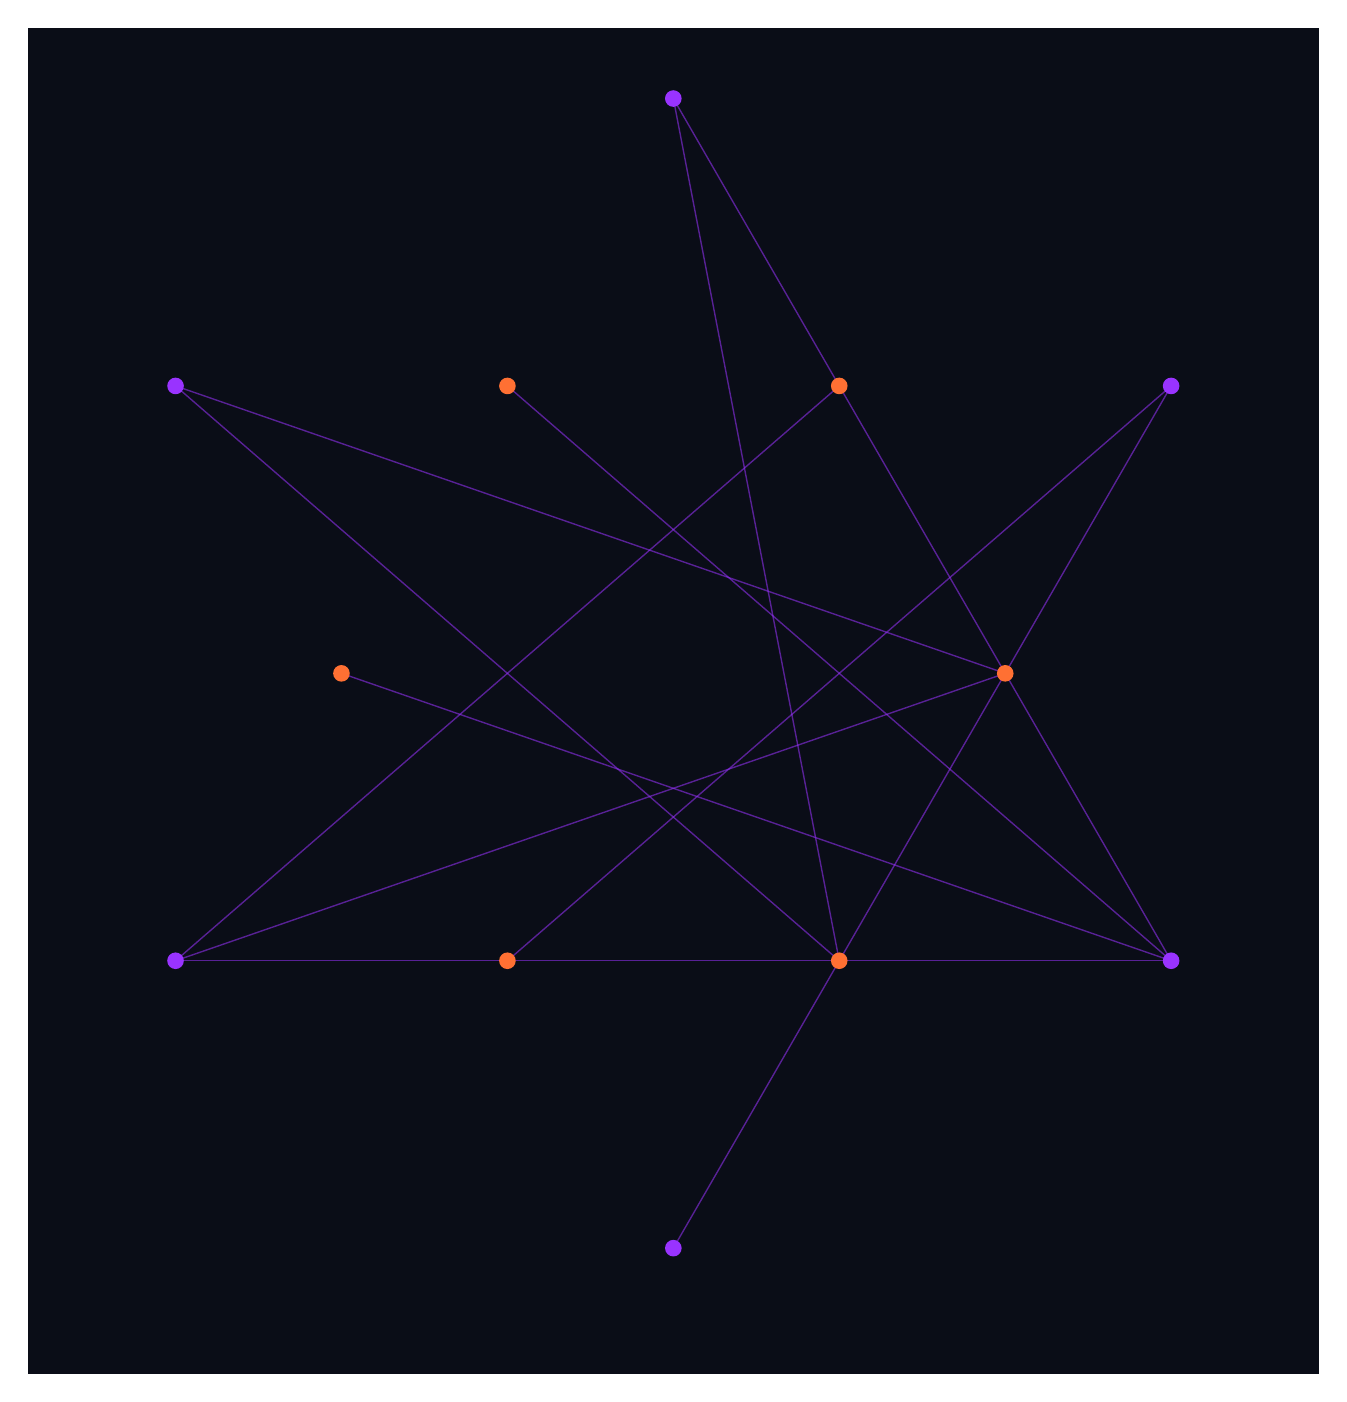
\begin{tikzpicture}
\definecolor{ring0}{rgb}{1.000,0.440,0.200}
\definecolor{ring1}{rgb}{0.600,0.200,1.000}
\definecolor{bg}{rgb}{0.04,0.05,0.09}
\fill[bg] (-8.2,-8.9) rectangle (8.2,8.2);
\draw[ring1,line width=0.5pt,opacity=0.55] (4.215,0.000)--(-6.322,-3.650);
\draw[ring1,line width=0.5pt,opacity=0.55] (4.215,0.000)--(-6.322,3.650);
\draw[ring1,line width=0.5pt,opacity=0.55] (2.107,-3.650)--(-6.322,3.650);
\draw[ring1,line width=0.5pt,opacity=0.55] (2.107,-3.650)--(-0.000,7.300);
\draw[ring1,line width=0.5pt,opacity=0.55] (-2.107,-3.650)--(6.322,3.650);
\draw[ring1,line width=0.5pt,opacity=0.55] (-4.215,-0.000)--(6.322,-3.650);
\draw[ring1,line width=0.5pt,opacity=0.55] (-2.107,3.650)--(6.322,-3.650);
\draw[ring1,line width=0.5pt,opacity=0.55] (2.107,3.650)--(-6.322,-3.650);
\draw[ring1,line width=0.5pt,opacity=0.55] (6.322,-3.650)--(-6.322,-3.650);
\draw[ring1,line width=0.5pt,opacity=0.55] (6.322,-3.650)--(-0.000,7.300);
\draw[ring1,line width=0.5pt,opacity=0.55] (0.000,-7.300)--(6.322,3.650);
\fill[ring0] (4.215,0.000) circle (3.0pt);
\fill[ring0] (2.107,-3.650) circle (3.0pt);
\fill[ring0] (-2.107,-3.650) circle (3.0pt);
\fill[ring0] (-4.215,-0.000) circle (3.0pt);
\fill[ring0] (-2.107,3.650) circle (3.0pt);
\fill[ring0] (2.107,3.650) circle (3.0pt);
\fill[ring1] (6.322,-3.650) circle (3.0pt);
\fill[ring1] (0.000,-7.300) circle (3.0pt);
\fill[ring1] (-6.322,-3.650) circle (3.0pt);
\fill[ring1] (-6.322,3.650) circle (3.0pt);
\fill[ring1] (-0.000,7.300) circle (3.0pt);
\fill[ring1] (6.322,3.650) circle (3.0pt);
\end{tikzpicture}
\end{document}